\section{Methodisches Vorgehen zur Problemlösung}

%%%%%%%%%%%%%%%%%%%%%%%%%%%%%%%%%%%%%%%%%%%%%%%%%%%%%%%%%%%%%%%%%%%%%%%%%%%%%%%%%%%%%%%%%%%%%%
\subsection{Aktueller Stand der Technologie}

\subsubsection{Bluetooth Low Energy}\label{sssec:BLE}

\subsubsection{Raspberry Pi}
Für die Zentrale und die DeSearch-Boxen ist zunächst eine Hardware-Entscheidung notwendig. Benötigt werden Mikrocontroller oder Mikrocomputer mit folgenden Eigenschaften:
\begin{itemize}
	\item W-LAN Verbindung von der Box zur Zentrale möglich
	\item Bluetooth-fähige Box zur Markenerkennung
	\item Zentrale muss als Server fungieren und HTTP-Requests senden und verarbeiten können
	\item Datenbank-Installation zur Datenhaltung notwendig
\end{itemize}
Zudem sollen die Kosten pro Gerät so gering wie möglich gehalten werden. \\
Der Rasberry Pi ist ein Mikrocomputer mit einer Grundfläche, die etwas größer ist als eine Kreditkarte. Die Anschaffungskosten liegen ohne Zubehör bei etwa 42 €. Für diese geringen Anschaffungskosten erhält man einen vollwertigen, Linux-Basierten Computer mit einer ARM-CPU, W-LAN und Bluetooth-Schnittstelle. Im Gegensatz zu Mikrocontrollern ist der Raspberry Pi leistungsfähiger und läuft stabiler \citep[Vgl.][S.35ff.]{raspi}. Auf einem Arduino beispielweise kann nur C++-Code in einer Endlos-Schleife ausgeführt werden. Der Pi hingegen bietet die Möglichkeit, Bash-Skripte, Python-Code, Datenbank-Anfragen und Webserver gleichzeitig auszuführen. Die Entscheidung für Raspberry Pi ist auch aufgrund der relativ niedrigen Anschaffungskosten für einen kompletten Rechner mit Betriebssystem gefallen. Für die Entwickler ist das Betriebssystem Linux zudem am einfachsten zu bedienen. Für das Projekt werden Pakete mit SD-Karte, W-LAN und Bluetooth-Dongles, Netzteil und Gehäuse für ca. 75 € pro Paket angeschafft.
\subsubsection{Authentifizierungstechnologie}
\subsubsection{Software-Rollout mit apt-get}
\subsubsection{PostgreSQL}


\subsection{Umsetzung der Anforderungen}

\subsubsection{Vernetzung der DeSearch-Boxen und Infrastruktur}
\subsubsection{User-Authentifizierung}
\subsubsection{Erkennen der Marken und Kommunikation zur Zentrale}
\subsubsection{Datenhaltung mittels PostgreSQL}
\subsubsection{Administrative Benutzeroberfläche}
\subsubsection{Installation der DeSearch-Boxen in der Testumgebung}
Die Raspberry Pi's werden in der DHBW Ravensburg am Campus Friedrichshafen zum Testbetrieb installiert. Dabei fungiert ein Pi als Zentrale und die anderen als DeSearch-Boxen, die die Funde an die Zentrale melden. In Tabelle \ref{tab:pis} ist eine Übersicht über alle installierten Raspberry Pi's aufgelistet.
Dazu wurde uns vom Netzwerkadministrator der DHBW die Erlaubnis eingeräumt, die vorhandene Infrastruktur zu verwenden. Daran geknüpft waren allerdings folgende Bedingungen bzw. Einschränkungen:
\begin{itemize}
	\item Zugriffe aus dem Internet sind nicht erlaubt.
	\item Alle Pi's außer der Zentrale (Slaves) verbinden sich über WLAN unter Verwendung unserer Zugangsdaten mit dem Netzwerk.
	\item Die Zentrale bekommt einen LAN Anschluss und eine feste IP Adresse plus DNS Eintrag zugewiesen.
	\item Ein Verbindungsaufbau zu den Slaves ist nicht möglich - jegliche Kommunikation muss von ihnen initiiert werden.
\end{itemize}
Die letzte Bedingung stelle eine Herausforderung dar, da damit auch kein SSH-Zugriff auf die DeSearch-Boxen möglich ist, der benötigt wird um die DeSearch Anwendung zu aktualisieren, starten oder überwachen.
Dieses Problem konnte gelöst werden, da mit der Zentrale ein Gerät im Netzwerk ist, das für alle anderen Pi's und auch die zur Entwicklung und Wartung verwendeten Laptops erreichbar ist, kann darüber ein Tunnel aufgebaut werden.
Zum Aufbauen des Tunnels hat sich die Verwendung der SSH Portforwarding Funktion angeboten, da alle beteiligten Geräte bereits für die Verwendung von SSH eingerichtet waren. Eine schematische Darstellung der Vorgehensweise finden sie in Abbildung \ref{fig:tunnel}.
Zum Verbindungsaufbau wurde ein technischer Benutzer mit dem Namen "tunnel" auf der Zentrale angelegt, der sich über SSH und Zertifikat Authentifizierung einloggen kann.
Jeder Slave hat einen RSA Schlüssel erhalten, den er zum Login verwenden kann, und über einen Eintrag ein der Crontabelle wird sichergestellt, dass der Tunnel immer offen gehalten wird.
Der Ausgangsport des Tunnels ist dabei für jede DeSearch-Box eindeutig. Soll nun eine Verbindung zu einer Box hergestellt werden, so muss erst eine SSH Verbindung zur Zentrale aufgebaut werden und dort eine SSH Verbindung zum Eingang des Tunnels (localhost plus Tunnel Ausgangport) hergestellt werden.
\begin{table}[h]
	\begin{tabular}{ | p{2,5cm} | p{2,5cm} | p{4cm} | p{6cm} |}
		\hline
		\textbf{Pi-Nummer} & \textbf{Funktion} & \textbf{Installationsort} &  \textbf{Erreichbarkeit} \\ \hline
		3 & Zentrale & Büro Herr Judt & statische IP 141.68.30.39 oder \mbox{Judt-Master.it.ba-ravensburg.de} \\ \hline
		5 & DeSearch-Box & Haupteingang oberhalb der Treppe & Tunnel über Zentrale, Port 19005 \\ \hline
		
	\end{tabular}
	\caption{Übersicht der Raspberry Pi's mit Funktion, Installationsort und Erreichbarkeit}
	\label{tab:pis}
\end{table}

\begin{figure}
	\centering
	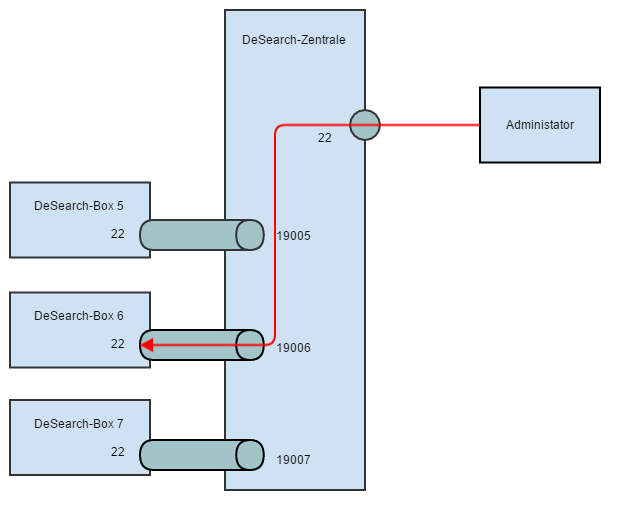
\includegraphics[width=\textwidth]{./images/tunnel.png}
	\caption[Schematische Darstellung der Verwendung des SSH Tunnels]{\textbf{Schematische Darstellung der Verwendung des SSH Tunnels} - Beispielhaft ist hier eine Verbindung vom Administrator zur DeSearch-Box 6 dargestellt (roter Pfeil).}
	\label{fig:tunnel}
\end{figure} 

